\documentclass[10pt]{article}

\usepackage{a4wide}
\usepackage[utf8]{inputenc}

\usepackage[percent]{overpic}
\usepackage{graphicx}
\usepackage{amsmath}
\usepackage{mathtools}
\usepackage{placeins}
\usepackage[osf,sc]{mathpazo}
\usepackage{listings}

\usepackage{xcolor}
\usepackage{listings}

\usepackage{amssymb}
\usepackage{url}
\usepackage[T1]{fontenc}
\usepackage[utf8]{inputenc}
%\global\language=5

\usepackage{textcomp}
\usepackage{setspace}
\usepackage{palatino}

\definecolor{mGreen}{rgb}{0,0.6,0}
\definecolor{mGray}{rgb}{0.5,0.5,0.5}
\definecolor{mPurple}{rgb}{0.58,0,0.82}
\definecolor{backgroundColour}{rgb}{0.95,0.95,0.92}

\lstdefinestyle{CStyle}{
    basicstyle=\ttfamily\footnotesize\setstretch{1},
    backgroundcolor=\color{backgroundColour},   
    commentstyle=\color{mGreen},
    keywordstyle=\color{magenta},
    numberstyle=\tiny\color{mGray},
    stringstyle=\color{mPurple},
    %basicstyle=\footnotesize,
    breakatwhitespace=false,         
    breaklines=true,                 
    captionpos=b,                    
    keepspaces=true,                 
    numbers=left,                    
    numbersep=5pt,                  
    showspaces=false,                
    showstringspaces=false,
    showtabs=false,                  
    tabsize=2,
    language=C
}

\renewcommand{\lstlistlistingname}{Code Listings}
\renewcommand{\lstlistingname}{Code Listing}
\definecolor{gray}{gray}{0.5}
\definecolor{green}{rgb}{0,0.5,0}

\pagestyle{empty}

%\parindent=0pt

\def\mvec#1{\mathbf{#1}}

\newcommand{\code}[1]{\textbf{\texttt{#1}}}
\newcommand{\tuchar}[0]{\code{uchar}}
\newcommand{\tfloat}{\code{float}}

\begin{document}

\section*{Introduction to OpenCV Library}

\begin{figure}[th]
\begin{center}
    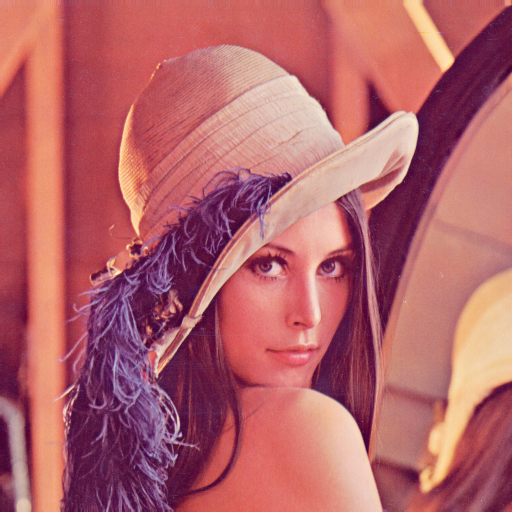
\includegraphics[width=0.3\textwidth]{lena} 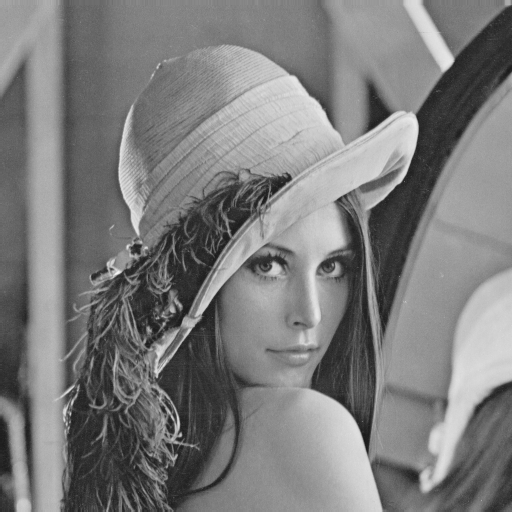
\includegraphics[width=0.3\textwidth]{lena_gray} 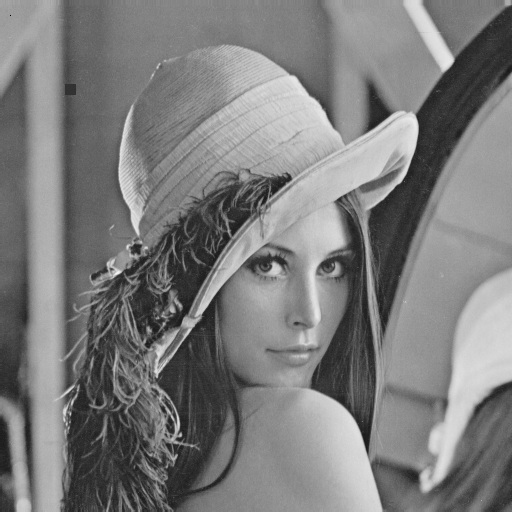
\includegraphics[width=0.3\textwidth]{gray_8uc1_img} 

    \caption{Color image of Lena, the most used image in digital image processing \textit{(left)};
    grayscale image of Lena \textit{(middle)}; grayscale image of Lena with modified pixel and drawn rectangle \textit{(right)}.}
    \label{img:lena}
\end{center}
\end{figure}

Welcome to the Digital Image Processing exercises\footnote{\texttt{http://mrl.cs.vsb.cz/people/gaura/dzo\_course}}.
In these exercises, we'll implement image processing algorithms that are discussed in lectures from the theoretical perspective.

Listing~\ref{lst:full} shows the full source code of our exercise that is able to load a color image,
convert it to grayscale image, read pixel values,
manipulate pixel values, and draw a rectangle. Let's go through the code in more detail.

OpenCV is a C++ library for manipulating images and contains a lot of image processing and analysis algorithms.
Most of the OpenCV's functions reside in the \code{cv} namespace.
Images are stored in matrices using \code{cv::Mat} data type.
To open an image, we use \code{cv::imread} function that returns an image that we can store in a variable.
Images can be color or grayscale. Most of our algorithms will use grayscale images.
The following code reads image in color and grayscale variant and stores them in two different variables.

\begin{lstlisting}[style=CStyle,caption={Reading image.},label={lst:read_image}]
// load color image from file system to cv::Mat variable, this will be loaded using 8 bits (uchar)
cv::Mat src_8uc3_img = cv::imread( "images/lena.png", CV_LOAD_IMAGE_COLOR );

// load color image from file system to cv::Mat variable, this will be loaded using 8 bits (uchar)
cv::Mat src_8uc1_img = cv::imread( "images/lena.png", CV_LOAD_IMAGE_GRAYSCALE );
\end{lstlisting}

As you can see, we now have the color version of Lena (Figure \ref{img:lena} (left)) and gray scale Lena (Figure \ref{img:lena} (middle))
loaded into variables \code{src\_8uc3\_img} and \code{src\_8uc1\_img}.

However, we can also convert images between different color spaces.
We can easily convert a RGB image to grayscale one using \code{cv::cvtColor}
function as shown in listing \ref{lst:cvtcolor}.

\begin{lstlisting}[style=CStyle,caption={Reading image.},label={lst:cvtcolor}]
// convert input color image to grayscale one, CV_BGR2GRAY specifies direction of conversion
cv::cvtColor( src_8uc3_img, gray_8uc1_img, CV_BGR2GRAY );
\end{lstlisting}

We just converted color image \code{src\_8uc3\_img} to empty image \code{gray\_8uc1\_img}.

When we load an image from a file, each pixel is represented using 8 bits of information (\code{unsigned char} in C++ that we can refer as
\code{uchar}\footnote{This is simplified, but OK for our needs}). Pixel values are in range 0 - 255. In grayscale image, we have one \code{uchar} per pixel.
In color image, we have three \code{uchar}s per pixel forming traditional \textbf{RGB} pixels.
However, for some image processing operations, it is better to represent image using values in range 0.0 - 1.0.
Such values have to stored in real value data type. For our use, it'll be completely sufficient to use \code{float} data type for such representation.
To convert a grayscale image from 8 bits (\code{uchar}) representation to 32 bits (\code{float}) representation we use \code{convertTo} method of \code{cv::Mat} variable.
The parameters of the method are: output image, output data type, and conversion scale and the method usage is described below.

\begin{lstlisting}[style=CStyle,caption={Reading image.},label={lst:convertto}]
// convert grayscale image from 8 bits to 32 bits, resulting values will be in the interval 0.0 - 1.0
gray_8uc1_img.convertTo( gray_32fc1_img, CV_32FC1, 1.0 / 255.0 );
\end{lstlisting}

Since the main aim of this course is to implement image processing algorithms, we'll need to access pixels of an image.
To do so, we'll us \code{at} method of the \code{cv::Mat} data type.
This method is templated (it needs a type specifier in angle brackets before arguments. Method signature is as follows.
\\
\code{at<image\_type>( int y, int x )}

\begin{lstlisting}[style=CStyle,caption={Accessing pixels.},label={lst:pixel-access}]
// read grayscale value of a pixel, image represented using 8 bits
uchar p1 = gray_8uc1_img.at<uchar>( y, x );

// read grayscale value of a pixel, image represented using 32 bits
float p2 = gray_32fc1_img.at<float>( y, x );

// read color value of a pixel, image represented using 8 bits per color channel
cv::Vec3b p3 = src_8uc3_img.at<cv::Vec3b>( y, x );

// print values of pixels
printf( "p1 = %d\n", p1 );
printf( "p2 = %f\n", p2 );
printf( "p3[ 0 ] = %d, p3[ 1 ] = %d, p3[ 2 ] = %d\n", p3[ 0 ], p3[ 1 ], p3[ 2 ] );
\end{lstlisting}

We're assigning a grayscale value (brightness) to the \tuchar{} variable \code{p1}.
\code{gray\_8uc1\_img} has brightness values represented using 8 bits. As you can see, type specifier
of \code{at} method is set to \tuchar{}. It's followed by \code{y}, and \code{x} variables that specify,
at which position to read pixel value.
The same procedure is done in the case of \code{gray\_32fc1\_img} image, which uses 32 bits representation
of brightness values. The only difference is that we use \tfloat{} instead of \tuchar{} data type.
To access color pixels in \code{src\_8uc3\_img}, we need to use \code{cv::Vec3b}.
This type holds three values (RGB) at once. To access each color value, we use \code{[]} notation as is used
in the above example.

Another important operation with image pixels is, of course, setting a new pixel brightness.
This is done again using \code{at} method. The only difference from the read operation is that we assign
a new value to the method. An example is shown in the listing below.

\begin{lstlisting}[style=CStyle,caption={Asigning a new value to a pixel.},label={lst:pixel-assign}]
// set pixel value to 0 (black)
gray_8uc1_img.at<uchar>( y, x ) = 0;
\end{lstlisting}

When implementing image processing algorithms, you'll quite often need to go through all image pixels
and perform some operation with brightness values. To access all pixels, we usually use two nested for loops
to iterate over all rows and in each row to iterate over all columns. As an example (\ref{lst:gradient-image}),
we'll create a gradient image.
First, we crate a new image \code{gradient\_8uc1\_img} with 50 rows and 256 columns and with \code{CV\_8UC1} type.
This means that image will use 8 bits as data representation (\tuchar{}) and one channel, so it's essentially
a grayscale image. Then we iterate over all pixels and assign brightness value according to the column number.

\begin{lstlisting}[style=CStyle,caption={Create an image of a horizontal gradient from black color to white using grayscale.},label={lst:gradient-image}]
// declare variable to hold gradient image with dimensions: width= 256 pixels, height= 50 pixels.
// Gray levels wil be represented using 8 bits (uchar)
cv::Mat gradient_8uc1_img( 50, 256, CV_8UC1 );

// For every pixel in image, assign a brightness value according to the x coordinate.
// This wil create a horizontal gradient.
for ( int y = 0; y < gradient_8uc1_img.rows; y++ ) {
    for ( int x = 0; x < gradient_8uc1_img.cols; x++ ) {
        gradient_8uc1_img.at<uchar>( y, x ) = x;
    }
}
\end{lstlisting}

\begin{figure}[th]
\begin{center}
    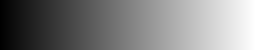
\includegraphics[width=0.5\textwidth]{gradient_8uc1_img}
    \caption{A gradient image produced by our code.}
    \label{img:gradient_example}
\end{center}
\end{figure}

You can find the full listing of the exercise's code below.

\begin{lstlisting}[style=CStyle,caption={Full exercise code.},label={lst:full}]
#include <iostream>

#include <opencv2/opencv.hpp>

int main( int argc, char *argv[] )
{
    cv::Mat src_8uc3_img = cv::imread( "images/lena.png", CV_LOAD_IMAGE_COLOR ); // load color image from file system to Mat variable, this will be loaded using 8 bits (uchar)
    //cv::imshow( "LENA", img );

    // declare variable to hold grayscale version of img variable, gray levels wil be represented using 8 bits (uchar)
    cv::Mat gray_8uc1_img;
    // declare variable to hold grayscale version of img variable, gray levels wil be represented using 32 bits (float)
    cv::Mat gray_32fc1_img;

    cv::cvtColor( src_8uc3_img, gray_8uc1_img, CV_BGR2GRAY ); // convert input color image to grayscale one, CV_BGR2GRAY specifies direction of conversion
    gray_8uc1_img.convertTo( gray_32fc1_img, CV_32FC1, 1.0 / 255.0 ); // convert grayscale image from 8 bits to 32 bits, resulting values will be in the interval 0.0 - 1.0

    int x = 10, y = 15; // pixel coordinates

    uchar p1 = gray_8uc1_img.at<uchar>( y, x ); // read grayscale value of a pixel, image represented using 8 bits
    float p2 = gray_32fc1_img.at<float>( y, x ); // read grayscale value of a pixel, image represented using 32 bits
    cv::Vec3b p3 = src_8uc3_img.at<cv::Vec3b>( y, x ); // read color value of a pixel, image represented using 8 bits per color channel

    // print values of pixels
    printf( "p1 = %d\n", p1 );
    printf( "p2 = %f\n", p2 );
    printf( "p3[ 0 ] = %d, p3[ 1 ] = %d, p3[ 2 ] = %d\n", p3[ 0 ], p3[ 1 ], p3[ 2 ] );

    gray_8uc1_img.at<uchar>( y, x ) = 0; // set pixel value to 0 (black)

    // draw a rectangle
    cv::rectangle( gray_8uc1_img, cv::Point( 65, 84 ), cv::Point( 75, 94 ),
                   cv::Scalar( 50 ), CV_FILLED );

    // declare variable to hold gradient image with dimensions: width= 256 pixels, height= 50 pixels.
    // Gray levels wil be represented using 8 bits (uchar)
    cv::Mat gradient_8uc1_img( 50, 256, CV_8UC1 );

    // For every pixel in image, assign a brightness value according to the x coordinate.
    // This wil create a horizontal gradient.
    for ( int y = 0; y < gradient_8uc1_img.rows; y++ ) {
        for ( int x = 0; x < gradient_8uc1_img.cols; x++ ) {
            gradient_8uc1_img.at<uchar>( y, x ) = x;
        }
    }

    // diplay images
    cv::imshow( "Gradient 8uc1", gradient_8uc1_img );
    cv::imshow( "Lena gray 8uc1", gray_8uc1_img );
    cv::imshow( "Lena gray 32fc1", gray_32fc1_img );

    cv::waitKey( 0 ); // wait until keypressed

    return 0;
}
\end{lstlisting}

\end{document}

